\chapter{Álgebra Lineal Esencial---The Geometry of Transformation}

\begin{quote}
	\itshape
	``Geometry is the art of correct reasoning from incorrectly drawn figures.''
	
	\raggedleft--- Henri Poincaré
\end{quote}

\section{Vectors as Directional Beings}

\begin{seanbox}{1.1}
	\textbf{Rigorous Definition:}
	
	A vector $\vect{x} \in \R^d$ is an element of $d$-dimensional Euclidean space, represented relative to a chosen basis $\{\vect{e}_j\}_{j=1}^d$ as:
	
	\begin{equation}
		\vect{x} = \sum_{j=1}^d x_j \vect{e}_j = \begin{bmatrix} x_1 \\ x_2 \\ \vdots \\ x_d \end{bmatrix}
	\end{equation}
	
	\textbf{Notational Conventions:}
	\begin{itemize}
		\item Boldface ($\vect{x}$): Coordinate-free vector (geometric object)
		\item Subscript ($x_j$): Component along $j$-th basis vector (coordinate representation)
		\item $\in \R^d$: Membership in vector space (ontological assertion)
	\end{itemize}
\end{seanbox}

\begin{philobox}
	\textbf{Philosophical Intuition:}
	
	A vector is not merely ``an array of numbers'' but a \textit{mode of directedness}---what Heidegger called \textit{Ausrichtung}. The notation $\vect{x} \in \R^d$ captures the profound relationship between:
	
	\begin{enumerate}
		\item The \textit{particular} ($\vect{x}$): A specific arrow in space
		\item The \textit{universal} ($\R^d$): The space of all possible directions
	\end{enumerate}
	
	The subscript $x_j$ is an \textit{index of determination}---it specifies which dimension of freedom is constrained. This echoes Aristotle's \textit{potentiality} vs. \textit{actuality}: $\R^d$ contains all potential vectors, $\vect{x}$ is one actualized instance.
\end{philobox}

\subsection{Historical Depth: From Grassmann to Geometric Intuition}

The modern concept of vector emerged from Hermann Grassmann's \textit{Ausdehnungslehre} (Theory of Extension, 1844), where he conceived vectors as \textit{extensive magnitudes}---entities possessing both direction and scale. Grassmann was heavily influenced by Kant's philosophy of space as a form of \textit{pure intuition} (Anschauung).

\begin{remark}[Grassmann's Philosophical Roots]
	In the \textit{Critique of Pure Reason} (1781), Kant argued that space is not an empirical concept derived from experience but an \textit{a priori} form that structures all outer intuition. Grassmann sought to develop an algebra that would capture this synthetic nature of spatial relations.
\end{remark}

The notation $\vect{x}$ (boldface) became standard with Josiah Willard Gibbs (1881), who developed vector calculus for physics. His choice of bold type was not arbitrary---it visually distinguishes geometric objects (vectors) from scalars, embodying the ontological difference between magnitude-with-direction and pure quantity.

\subsection{The Inner Product as Measure of Alignment}

\begin{seanbox}{1.2}
	\textbf{Inner Product:}
	
	For $\vect{x}, \vect{y} \in \R^d$:
	\begin{equation}
		\langle \vect{x}, \vect{y} \rangle = \vect{x}^\top \vect{y} = \sum_{j=1}^d x_j y_j = \|\vect{x}\| \|\vect{y}\| \cos\theta
	\end{equation}
	
	where $\theta$ is the angle between vectors.
	
	\textbf{Notational Choices:}
	\begin{itemize}
		\item Angle brackets $\langle \cdot, \cdot \rangle$: Abstract inner product (basis-independent)
		\item Transpose $\vect{x}^\top \vect{y}$: Matrix notation (computation-friendly)
		\item Summation $\sum x_j y_j$: Einstein convention (index-level detail)
	\end{itemize}
\end{seanbox}

\begin{visualbox}
	\textbf{Geometric Intuition:}
	
	\begin{center}
		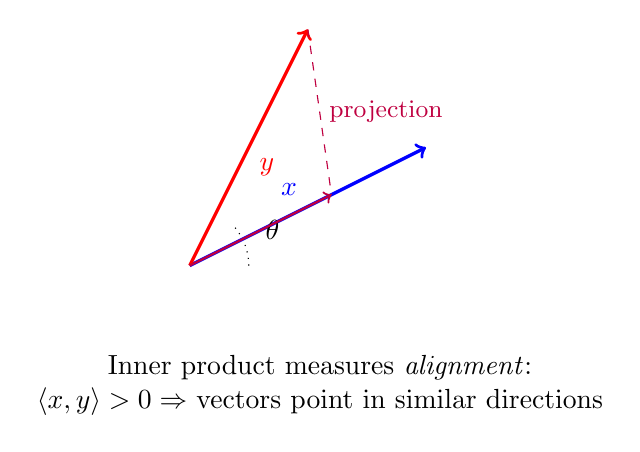
\begin{tikzpicture}[scale=1.5]
			% Origin
			\coordinate (O) at (0,0);
			
			% Vectors
			\draw[->, very thick, blue] (O) -- (2,1) node[midway, above left] {$\vect{x}$};
			\draw[->, very thick, red] (O) -- (1,2) node[midway, below right] {$\vect{y}$};
			
			% Angle
			\draw[dotted] (0.5,0) arc (0:45:0.5);
			\node at (0.7, 0.3) {$\theta$};
			
			% Projection
			\draw[dashed, purple] (1,2) -- (1.2,0.6) node[midway, right] {\small projection};
			\draw[->, thick, purple] (O) -- (1.2,0.6);
			
			\node[below=1cm, align=center] at (current bounding box.south) {
				Inner product measures \textit{alignment}:\\
				$\langle \vect{x}, \vect{y} \rangle > 0 \Rightarrow$ vectors point in similar directions
			};
		\end{tikzpicture}
	\end{center}
\end{visualbox}

\begin{philosophical}
	The inner product is the mathematical formalization of \textit{resonance}---how much two directions ``agree.'' In Spinoza's \textit{Ethics}, the \textit{conatus} (striving) of each being either aligns or conflicts with others. The inner product quantifies this alignment:
	
	\begin{itemize}
		\item $\langle \vect{x}, \vect{y} \rangle > 0$: Constructive interference (harmony)
		\item $\langle \vect{x}, \vect{y} \rangle = 0$: Orthogonality (independence)
		\item $\langle \vect{x}, \vect{y} \rangle < 0$: Destructive interference (opposition)
	\end{itemize}
\end{philosophical}

\section{Matrices as Morphisms of Space}

\begin{seanbox}{1.3}
	\textbf{Matrix as Linear Transformation:}
	
	A matrix $\mat{A} \in \R^{m \times n}$ defines a linear map:
	\begin{equation}
		\mat{A}: \R^n \to \R^m, \quad \vect{y} = \mat{A}\vect{x}
	\end{equation}
	
	\textbf{Component-wise:}
	\begin{equation}
		y_i = \sum_{j=1}^n A_{ij} x_j \quad (\text{Einstein summation: } y_i = A_{ij} x_j)
	\end{equation}
	
	\textbf{Notational Philosophy:}
	\begin{itemize}
		\item First index ($i$): Output coordinate (codomain)
		\item Second index ($j$): Input coordinate (domain)
		\item Repeated index ($j$): Summation (contraction)
	\end{itemize}
\end{seanbox}

\subsection{The Matrix-Vector Product as Weighted Synthesis}

Each output component $y_i$ is a \textit{weighted sum} of all input components:
\begin{equation}
	y_i = A_{i1} x_1 + A_{i2} x_2 + \cdots + A_{in} x_n
\end{equation}

The weights $A_{ij}$ encode \textit{how much input $j$ contributes to output $i$}. This is not passive transmission but active \textit{synthesis}---the matrix constructs new information from old.

\begin{philosophical}
	In Kant's \textit{Critique of Pure Reason}, synthesis is the act by which the mind combines representations to produce knowledge. The matrix-vector product is mathematical synthesis:
	
	\begin{center}
		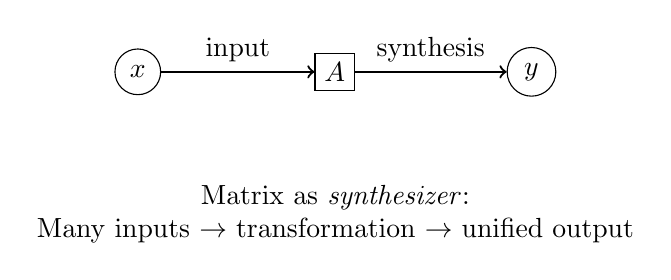
\begin{tikzpicture}[node distance=2.5cm]
			\node[draw, circle] (x) {$\vect{x}$};
			\node[draw, rectangle, right of=x] (A) {$\mat{A}$};
			\node[draw, circle, right of=A] (y) {$\vect{y}$};
			
			\draw[->, thick] (x) -- (A) node[midway, above] {input};
			\draw[->, thick] (A) -- (y) node[midway, above] {synthesis};
			
			\node[below=1cm, align=center] at (current bounding box.south) {
				Matrix as \textit{synthesizer}: \\
				Many inputs $\to$ transformation $\to$ unified output
			};
		\end{tikzpicture}
	\end{center}
\end{philosophical}

\subsection{Basis Change as Perspectival Transformation}

\begin{seanbox}{1.4}
	\textbf{Change of Basis:}
	
	Given a new basis specified by matrix $\mat{P}$ (columns are new basis vectors), the same vector has different coordinates:
	\begin{equation}
		\vect{x}_{\text{new}} = \mat{P}^{-1} \vect{x}_{\text{old}}
	\end{equation}
	
	Inversely:
	\begin{equation}
		\vect{x}_{\text{old}} = \mat{P} \vect{x}_{\text{new}}
	\end{equation}
\end{seanbox}

\begin{example}[Rotation as Basis Change]
	Rotating by $\theta$ counterclockwise:
	\begin{equation}
		\mat{R}(\theta) = \begin{bmatrix}
			\cos\theta & -\sin\theta \\
			\sin\theta & \cos\theta
		\end{bmatrix}
	\end{equation}
	
	The same geometric vector $\vect{x}$ has coordinates:
	\begin{itemize}
		\item $\vect{x}_{\text{original}}$ in the original basis
		\item $\vect{x}_{\text{rotated}} = \mat{R}(-\theta) \vect{x}_{\text{original}}$ in the rotated basis
	\end{itemize}
\end{example}

\begin{visualbox}
	\begin{center}
		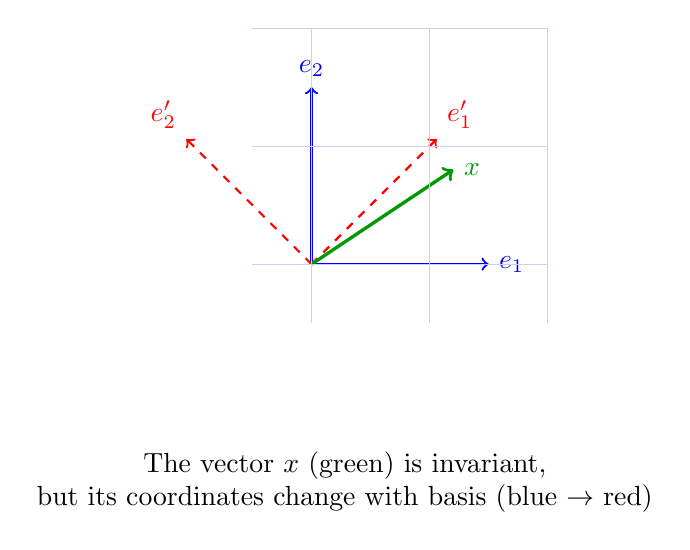
\begin{tikzpicture}[scale=1.5]
			% Original basis
			\draw[->, thick, blue] (0,0) -- (1.5,0) node[right] {$\vect{e}_1$};
			\draw[->, thick, blue] (0,0) -- (0,1.5) node[above] {$\vect{e}_2$};
			
			% Rotated basis
			\draw[->, thick, red, dashed] (0,0) -- (1.06,1.06) node[above right] {$\vect{e}'_1$};
			\draw[->, thick, red, dashed] (0,0) -- (-1.06,1.06) node[above left] {$\vect{e}'_2$};
			
			% A vector
			\draw[->, very thick, green!60!black] (0,0) -- (1.2,0.8) node[right] {$\vect{x}$};
			
			% Grid
			\draw[help lines, blue!20] (-0.5,-0.5) grid (2,2);
			
			\node[below=1.5cm, align=center] at (current bounding box.south) {
				The vector $\vect{x}$ (green) is invariant,\\
				but its coordinates change with basis (blue $\to$ red)
			};
		\end{tikzpicture}
	\end{center}
\end{visualbox}

\begin{philobox}
	\textbf{Kant's Copernican Revolution:}
	
	In the \textit{Critique of Pure Reason}, Kant inverted the traditional view: instead of our knowledge conforming to objects, objects conform to our modes of cognition. Similarly, vectors don't have ``true'' coordinates---coordinates are \textit{representations relative to a chosen frame}.
	
	This is the philosophical essence of basis change: \textbf{reality is perspectival}, yet geometric relationships (lengths, angles) are \textit{invariant}---they don't depend on coordinate choice.
\end{philobox}

\section{Tensors as Multi-Indexed Assemblages}

\begin{seanbox}{1.5}
	\textbf{Tensor Definition:}
	
	A tensor $\ten{T} \in \R^{I \times J \times K}$ is a multi-dimensional array:
	\begin{equation}
		\ten{T} = [T_{ijk}], \quad i \in \{1,\ldots,I\}, j \in \{1,\ldots,J\}, k \in \{1,\ldots,K\}
	\end{equation}
	
	\textbf{Special Cases:}
	\begin{itemize}
		\item 0th-order tensor: Scalar (no indices)
		\item 1st-order tensor: Vector (one index)
		\item 2nd-order tensor: Matrix (two indices)
		\item $n$th-order tensor: $n$ indices
	\end{itemize}
\end{seanbox}

\begin{example}[Images as Tensors]
	An RGB image is a 3rd-order tensor $\ten{I} \in \R^{H \times W \times 3}$:
	\begin{itemize}
		\item $I_{hwc}$: Pixel value at height $h$, width $w$, channel $c$ (R/G/B)
		\item Indices have \textit{semantic meaning}: $h,w$ are spatial, $c$ is chromatic
	\end{itemize}
\end{example}

\begin{philosophical}
	Deleuze's concept of \textit{assemblage} (agencement): a heterogeneous multiplicity where components retain their distinctness while forming a whole. A tensor is a mathematical assemblage---indices mark different ``lines of variation,'' each with its own semantic role.
	
	The notation $T_{ijk}$ makes this multiplicity explicit: we can ``slice'' along any index to extract sub-structures (fixing $k$ gives a matrix $T_{\cdot\cdot k}$).
\end{philosophical}

\subsection{Einstein Summation and Index Contraction}

\begin{seanbox}{1.6}
	\textbf{Einstein Summation Convention:}
	
	Repeated indices are implicitly summed:
	\begin{equation}
		y_i = A_{ij} x_j \equiv y_i = \sum_{j} A_{ij} x_j
	\end{equation}
	
	\textbf{General Tensor Contraction:}
	\begin{equation}
		C_{ik} = A_{ij} B_{jk} \quad \text{(matrix product)}
	\end{equation}
	\begin{equation}
		s = A_{ij} B_{ij} \quad \text{(Frobenius inner product)}
	\end{equation}
\end{seanbox}

\begin{codebox}
	\textbf{NumPy's einsum: Notation as Code}
	
	\begin{lstlisting}
		import numpy as np
		
		# Matrix-vector product: y_i = A_ij x_j
		A = np.random.randn(3, 4)
		x = np.random.randn(4)
		y = np.einsum('ij,j->i', A, x)
		
		# Batch matrix multiplication: C_bik = A_bij B_bjk
		A_batch = np.random.randn(10, 3, 4)  # 10 matrices, 3x4 each
		B_batch = np.random.randn(10, 4, 5)  # 10 matrices, 4x5 each
		C_batch = np.einsum('bij,bjk->bik', A_batch, B_batch)
		
		print(f"Shape of C: {C_batch.shape}")  # (10, 3, 5)
	\end{lstlisting}
	
	\textbf{Philosophical Insight:} The einsum string \texttt{'ij,j->i'} \textit{is} the mathematical notation $y_i = A_{ij} x_j$ in executable form. Notation and computation converge.
\end{codebox}

\section{Reflective Exercises}

\begin{exercise}
	Contemplate the difference between $x^{(i)}$ (superscript) and $x_i$ (subscript). Why do we write sample indices as superscripts and feature indices as subscripts? Does this notational choice reflect an ontological commitment (samples as instances of a universal, features as attributes of particulars)?
\end{exercise}

\begin{exercise}
	Consider the identity matrix $\mat{I}$. Its action is $\mat{I}\vect{x} = \vect{x}$---no change. Philosophically, $\mat{I}$ is \textit{pure self-relation}. How does this connect to Hegel's concept of identity as \textit{identity-in-difference}?
\end{exercise}

\begin{exercise}[Code Meditation]
	Run the following code and observe:
	\begin{lstlisting}
		import numpy as np
		
		x = np.array([1, 0])  # Unit vector along x-axis
		theta = np.pi / 4     # 45 degrees
		R = np.array([[np.cos(theta), -np.sin(theta)],
		[np.sin(theta),  np.cos(theta)]])
		
		x_rotated = R @ x
		print(f"Original: {x}")
		print(f"Rotated: {x_rotated}")
	\end{lstlisting}
	
	The \textit{same} geometric vector has coordinates $[1, 0]$ in one frame and $[\sqrt{2}/2, \sqrt{2}/2]$ in another. What does this teach about the nature of mathematical objects?
\end{exercise}
